%\documentclass{article}
%\usepackage[a4paper, total={6in, 8in}]{geometry}
\documentclass[reprint,amsmath,amssymb,rmp,onecolumn,notitlepage,11pt]{revtex4-1}
\usepackage[utf8]{inputenc}
%\usepackage{authblk}
%\usepackage{natbib}
\usepackage[normalem]{ulem}
\usepackage{graphicx}
\usepackage{hyperref}
\usepackage{xcolor}
\newcommand{\red}[1]{\textcolor{red!80!black}{#1}}
\newcommand{\blue}[1]{\textcolor{blue!80!black}{#1}}
\newcommand{\green}[1]{\textcolor{green!70!black}{#1}}
\newcommand{\gray}[1]{\textcolor{gray!80!black}{#1}}
\usepackage{mathtools}
\DeclarePairedDelimiter{\evdel}{\langle}{\rangle}
\usepackage[colorinlistoftodos]{todonotes}

\begin{document}
\title{The role of geometry in the chain separation distribution of links in protein contact networks}
\title{\red{We need a better title, the old one is too long} \green{Yes! But no better ideas at the moment}}
\title{\red{Chain separation distribution in protein contact networks}}
%\title{}
\author{Nora Molkenthin}
\affiliation{Potsdam Institut für Klimafolgenforschung}
\affiliation{Center for Advancing Electronics Dresden (cfaed), Technical University of Dresden}
\author{Steffen Mühle}
\affiliation{Uni Göttingen, 37077 Göttingen, Germany}
\author{Antonia S J S Mey}
\email[Electronic Address: ]{antonia.mey@ed.ac.uk}
\affiliation{EaStCHEM School of Chemistry, University of Edinburgh, Edinburgh, United Kingdom}
%\author{Marc Timme}
% \affiliation{Network Dynamics, Max Planck Institute for Dynamics and Self-Organization (MPIDS), 37077 Göttingen, Germany}
% \affiliation{Chair for Network Dynamics, Institute for Theoretical Physics and Center for Advancing Electronics Dresden (cfaed), Technical University of Dresden, 01069 Dresden}

\begin{abstract}
The distribution of chain separations of interacting amino acids in proteins roughly follows a power law. Here we show, analytically and in simulations, that a geometrical stochastic model of folding chains can explain this behaviour. 
\end{abstract}
\maketitle

\section*{Introduction}
Proteins, the molecular machines of every living organism perform vital tasks required for life to persist, ranging from transport (e.g. hemoglobin), signal transduction (e.g. rhodopsin), immune responses (e.g. antibodies), and hormonal regulation (e.g. insulin)~\cite{something}. All natural proteins are made up of 20 different amino acids which dictate the three dimensional conformations the proteins adopt in order to function~\cite{stuff}. One way of looking at the functional forms of proteins and classifying their structural properties is by looking at protein residue or contact networks~\cite{Vendruscolo2002,DiPaola2013,Estrada2011}. Protein Contact Networks (PCN), have shown promise in understanding protein folding patterns as well as revealing allosteric communication pathways~\cite{https://pubs.acs.org/doi/10.1021/acs.jcim.9b00320, and others}. 
From a physicist perspective it is interesting to understand the emergent behaviour in protein structure from PCNs, by investigating common network measures and their behaviour for PCNs. For example Bartoli et al.~\cite{bartoli2008effect} build a model in which they assume that proteins have a sequence separation distribution that follows $\frac{1}{\ell}$, where $\ell$ is the separation of two connected amino acids along the backbone chain as the simplest implementation of a connection probability, that decreases with the distance along the sequence. However, they do not provide a quantitative explanation for this assumption. 

Here, we show how a simple geometrical model can reproduce this heuristically found behaviour well, even providing a simple analytical approximation. The analytical approximation and geometrical model build on the idea that inherently geometrical objects, such as amino acids, imply that any resulting PCN network ensemble modelling them has to be spatially embedded~\cite{molkenthin2016scaling, molkenthin2020self}. 
Different approaches have been used in the past for geometrical models describing protein folding, some of which derived characteristics of the secondary structure from constraints on bond and torsion angles~\cite{maybe cite Flory stuff here as well?,Danielsson2010,Molkenthin2011} and others focused on the formation mechanisms of the tertiary structure~\cite{molkenthin2016scaling, molkenthin2020self}. 

Based on such considerations, the network formation process, repeatedly \red{(this may not be the adverb i'm looking for, but subsequently also doesnt quite work)} connects random pairs of units, without causing any intersections along the chain ~\cite{molkenthin2016scaling}. Such a model can now be used to investigate the emergent behaviour of sequence separation distributions as observed by Bartoli et al.~\cite{bartoli2008effect}. To this end, we analyze the sequence separation distributions that emerge from the geometric model, where the \emph{sequence separation} $\ell$ of a link is defined as the distance of the two end units along the original chain.
This is then compared to the sequence separation distribution extracted from protein residue networks (PRN) generated from protein data bank data. 

\red{We find that, despite the highly simplified model, the generated sequence distance distribution is in agreement with the one observed in networks generated from PDB data and roughly consistent with the heuristic $1/\ell$ finding. The analytical approximation provides a correction term on top of the $1/\ell$ heuristic.}


\section*{Protein Residue Networks and their synthetic counterparts}
The complex interaction pattern between the amino acids in a protein can be very naturally expressed as a network, in which each amino acid is represented by a node and spatial proximity is encoded as a link. Whenever two central $C_\alpha$ atoms are closer together than a threshold $d_c$, they are connected. These connections are encoded in the adjacency matrix of the folded protein, which is the binary matrix
\begin{equation}
  A^{\textsf{PDB}}_{ij}=
  \begin{cases}
   0, & \text{ if } d_{i,j}>d_c \text{ or } i=j\\
      1, & \text{ if } d_{i,j}\leq d_c .
      \end{cases}
    \label{eq:aij}
\end{equation}
Adjacency matrices are commonly used to describe networks and in this case represent the PRN.

The underlying formation mechanisms of individual protein folds are incredibly complex and depend on the surrounding solvent as well as the specific amino acid sequence and their quantum-mechanical interactions. Here we want to study the ensemble of all proteins, however, and will thus "average out" such specifics.

Based on the basic assumption that amino acids are objects in space, that can not overlap indefinitely, we introduced a model in \cite{molkenthin2020self} starting from a chain of identical spheres, each in contact only with the neighbours it is connected to. Then additional connections form by randomly selecting two spheres and moving them towards each other until they touch, the new links formed that way can not be broken in later steps and function as constraints on subsequent links. If contact of the two selected spheres is geometrically impossible without breaking previously made connections or leading to overlaps of any spheres, the link is not made and taken out of the pool of possible connections. This process is repeated until no more links can be formed without violating the geometric constraints.

In \cite{molkenthin2016scaling}, we have introduced a simplified, two-dimensional version of this model, which starts from a closed chain of $N$ unit discs and subsequently adds links, such that connected discs touch, yet no discs intersect. The advantage of this model is, that it can be approximated by a purely topological simplification, which can be treated analytically.

The topological constraints in the resulting network model are:
(a) New links always form between two units that are part of the same face of the graph (region enclosed by a cycle in the network). This prevents the overlapping of discs. (b) No links form across the outer face. This prevents the enclosure of a unit by less than six other units (which is geometrically impossible) such that. (c) The maximum degree of each unit is six, as six is the maximum number of unit discs, one central unit disc can touch. (d) Once connected by a link, pairs of units do not disconnect.

\section*{Analytic approximation}
Here we want to analytically approximate the sequence separation distribution for the simplified 2D model, that is the separation along the backbone chain of two nodes connected by a link, as illustrated in Fig~\ref{fig:schematic}~a).

\begin{figure}[h]
    \centering
    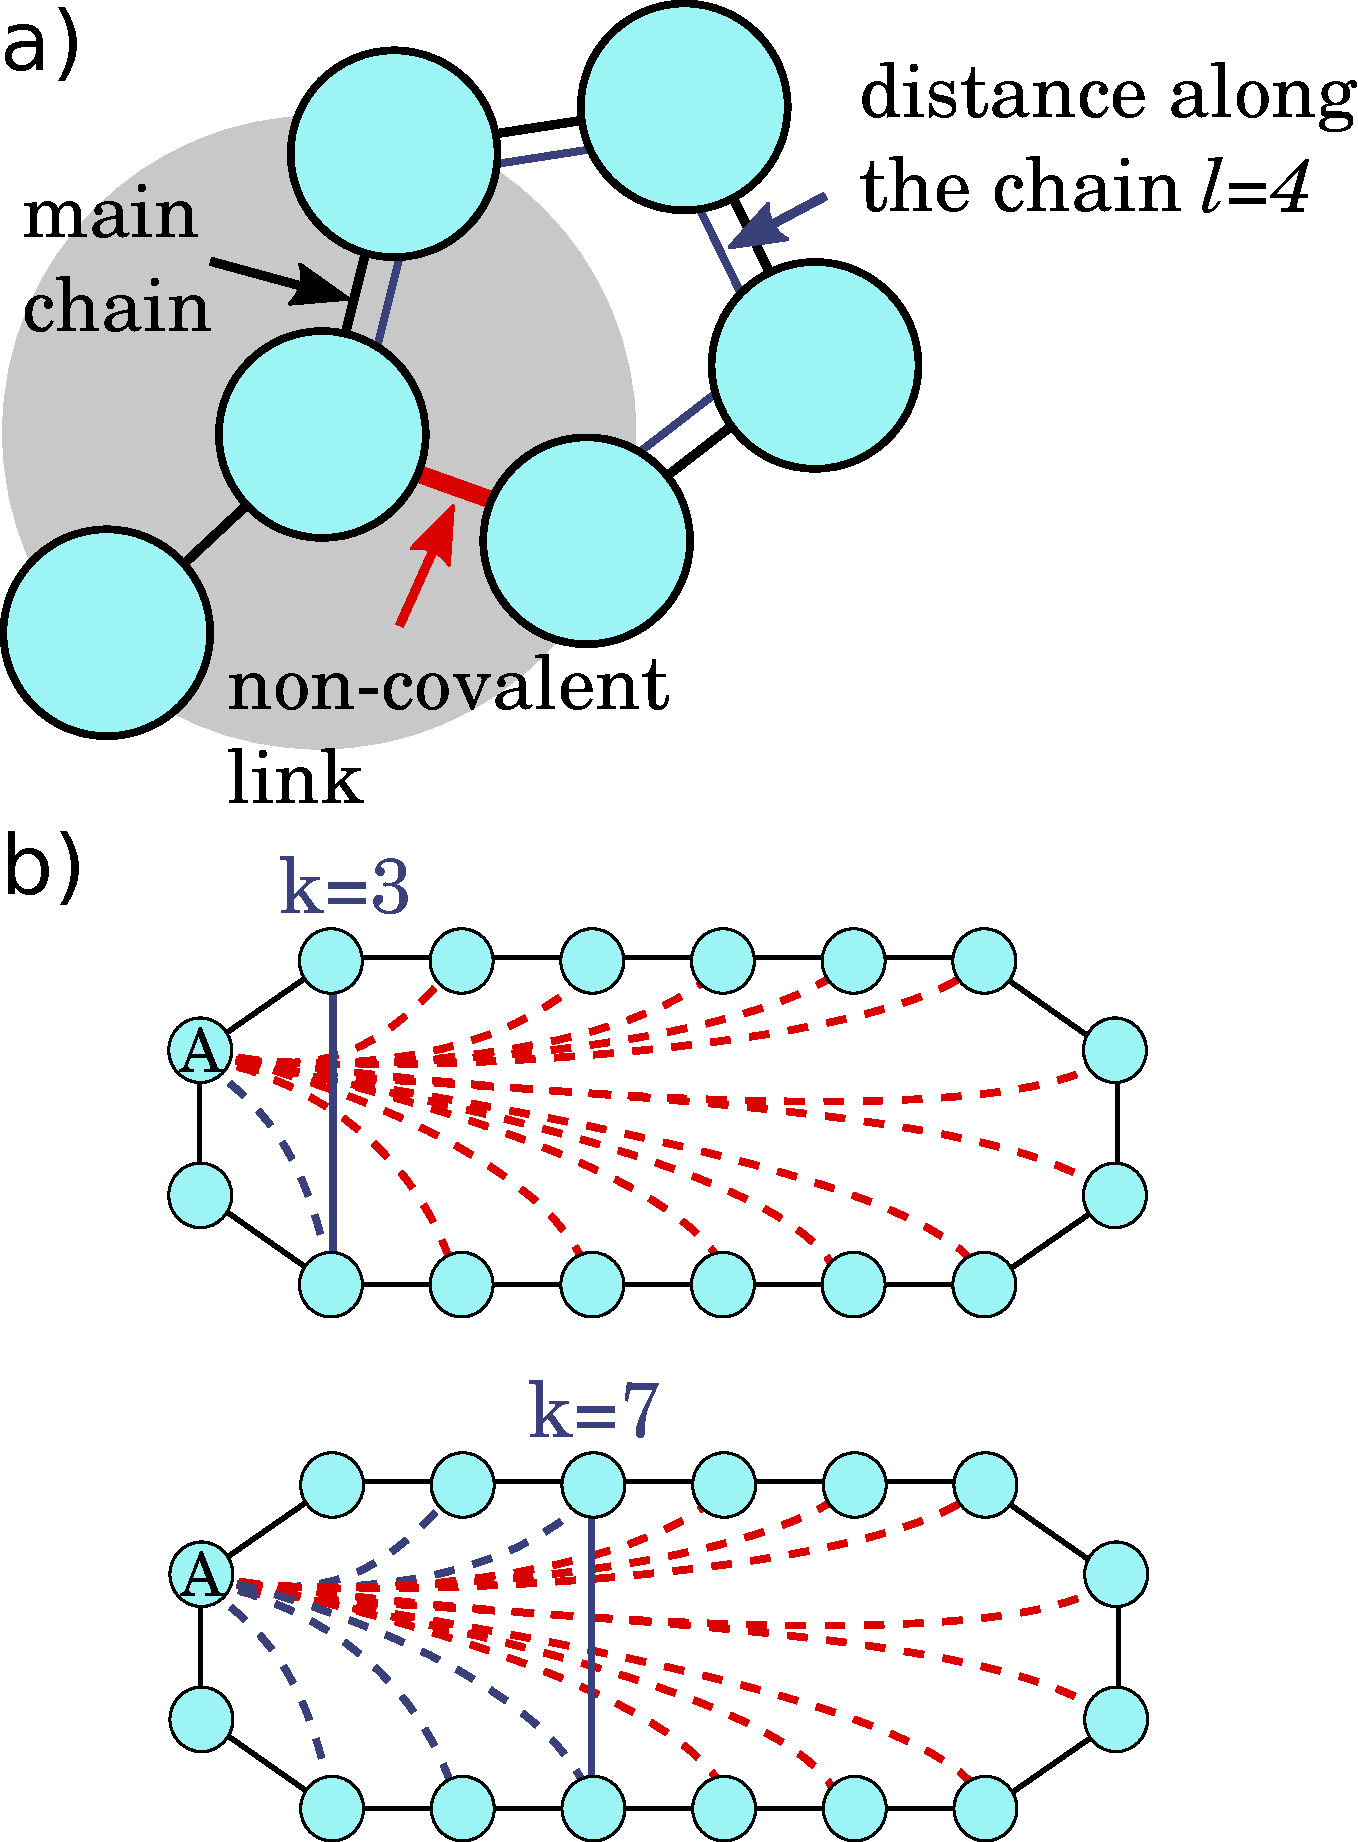
\includegraphics[width=0.4\columnwidth]{figures/Fig1.pdf}
    \caption{a) The sequence separation distribution is defined as the separation along the chain (blue) of two connected units (red). b) The solid blue link prohibits some connections from node $A$ (dotted red), while others are still permitted (dotted blue). Counting all newly excluded links, we find that a link of length $k$ prohibits $2(l-1)$ links of length $l$ up to a maximum of $k$ and $2(k-1)$ links of length $k$ or more.}
    \label{fig:schematic}
\end{figure}

Let us start by introducing the auxiliary variable $F(s)$, defined to be the number of possible links with a sequence separation of $s$. Before any links are added all sequence separations are equally likely, as there are $N$ possibilities of making a link of each separation $s$ with $2\leq s < N/2$.

As we add more links, not only are links taken out of this pool, because they have already been realized, each existing link can also geometrically prohibit other connections. Adding a link of length $s_1$ prohibits $2(s-1)$ links of length $s<s_1$ and $2(s_1-1)$ links of length $s>s_1$ (see Fig.~\ref{fig:schematic}~b). To find the expected number of links still available in subsequent stops, we average over all possible sequence separations $s_1$ of the first link added.

The expected distribution of possible links after one step is given thus by the average over available link pools taken over all possible lengths of the initial link
\begin{equation}
    F_1(s)= \frac{1}{N/2-2} \sum_{s_1=2}^{N/2} { \begin{cases}
    N-2(s-1) \text{ , for } s<s_1\\
    N-2(s_1 -1)\text{ , for } s\geq s_1
    \end{cases}}.
\end{equation}
Here we denote the size of the pool of available links after $i$ links have been added $F_i(s)$.

In subsequent steps we get the same reduction but starting from the pool $F_{k-1}(s)$ of the step before rather than the full $N$ links for each length. The reduction also needs to be multiplied by a factor 
\begin{equation}
    P_k(s)=\frac{F_k(s)}{C_k},
    \label{eq.Pk}
\end{equation}
with $C_k=\sum_{s=2}^{N/2}F^k(s)$, to only remove links that are still in the pool. This leads to the recursion
\begin{equation}
    F_k(s)= \frac{1}{N/2-2} \sum_{s_k=2}^{N/2} {\begin{cases}
     F_{k-1}(s)-2(s-1) P_{k-1}(s) \text{ , for } s<s_k\\
     F_{k-1}(s)-2(s_k -1)P_{k-1}(s)\text{ , for } s\geq s_k
    \end{cases}},
\end{equation}
which can be simplified to
\begin{align}
   F_k(s)&= \frac{1}{\frac{N}{2}-2} \frac{F_{k-1}(s)}{C_{k-1}}\left( \sum_{s_k=2}^{N/2}C_{k-1} - \sum_{s_k=2}^{s} 2(s_k-1) - \sum_{s_k=s+1}^{N/2} 2(s -1) \right) \nonumber \\
   &= \frac{1}{\frac{N}{2}-2}\frac{F_{k-1}(s)}{C_{k-1}}\left(\left(\frac{N}{2}-2\right)C_{k-1} -(s^2-s)-2\left(\frac{N}{2}-(s+1)\right)(s-1)\right)  \nonumber \\
   &= F_{k-1}(s)\left(1-\frac{-s^2 +(N-1)s-(N+1)}{(\frac{N}{2}-2)C_{k-1}} \right)\nonumber \\
   &=F_{k-1}(s)\left(1-\frac{f(s)}{(\frac{N}{2}-2)C_{k-1}} \right)
   \label{eq.Fk_rec}
\end{align}
Where we defined $f(s)=-s^2 +(N-1)s-(N+1) \approx N s - s^2 - N$ for notational brevity.

We can now use the recursive expression Eq.~\ref{eq.Fk_rec} to write down a closed expression for $F_k(s)$

\begin{equation}
    F_k(s)=N\prod_{i}^k\left(1-\frac{f(s)}{(\frac{N}{2}-2)C_{i-1}} \right)
\end{equation}

The probability distribution of the realized sequence separations of all added links is then given by the average over the available pools at each link addition step, leading to
\begin{align}
    P(s)&=\frac{1}{N-3}\sum_{k=0}^{N-3} P_k(s) \nonumber \\
    &= \frac{N}{N-3}\sum_{k=0}^{N-3} \frac{1}{C_k}\prod_{i}^k\left(1-\frac{f(s)}{(\frac{N}{2}-2)C_{i-1}} \right),
\end{align}
which makes use of Eq.~\ref{eq.Pk}. The only unknown in this expression is $C_k$, which we can not compute exactly. However, since $C_k$ monotonically decreases with $k$, $N>C_k>C_{N-2}$ always holds and we can obtain an upper and lower bound by replacing all $C_k$ in the expression with either $N$ (underestimates all probabilities) or $C_{N-2}$ (overestimates all probabilities). Each time we get an expression of the form 
\begin{align}
     P(s)&\approx\frac{N}{N-3}\sum_{k=0}^{N-3} \frac{1}{C_k}\prod_{i}^k\left(1-\frac{f(s)}{(\frac{N}{2}-2)C} \right)\nonumber \\
     &=\frac{N}{N-3} \sum_{k=0}^{N-3}\frac{1}{C_k}\left(1-\frac{f(s)}{(\frac{N}{2}-2)C} \right)^k \nonumber \\
     &\approx \frac{A}{f(s)}
\end{align}
for $1<s<\frac{N}{2}$,
where $A$ is an unknown constant, containing an approximation of the various normalization constants $C_i$, as well as the direct effects of the chain length. 
Since for long chains, $f(s)$ is largely dominated by the linear term, the distribution is well approximated by a power law with an exponent of $-1$. We have made use of the geometric series to approximately find a closed solution. 

In the last step of this approximation, we take the $C_k$ to all be approximately equal in order to apply the geometric series. However, in reality we know $1/C_k$ to increase with $k$, giving large $k$ summands relatively more weight than in a geometric series. This would lead to a correction in the exponent.

\begin{equation}
    P_{corrected}(s)\approx A f(s)^{-1+\alpha},
\end{equation}
where $0<\alpha<<1$ \red{, I think this is because we want $\alpha$ to be a small correction, so in fact we'd want it to be much smaller than 1}.


\section*{Data and simulations}
 For large values of the chain length $N$ we thus find an approximate power law probability distribution for the sequence separation with an exponent of $-1+\alpha$. Here we use simulations, as introduced in \cite{molkenthin2020self} and networks extracted from measured protein data from the PDB \cite{PDB} to compare this behaviour in realistic 3D settings and show that the basic principle persists, indicating that the sequence distance separation distribution is largely determined by simple geometric constraints.
 
 \red{write about how we picked out the specific structures to analyze, (i think we established that 200 to 400 is a very common range of lengths for proteins and i guess we will select them randomly, drawing from "typical" proteins or something), mention how many structures were analyzed and all that stuff.}
 
\begin{figure}[h]
        \centering
	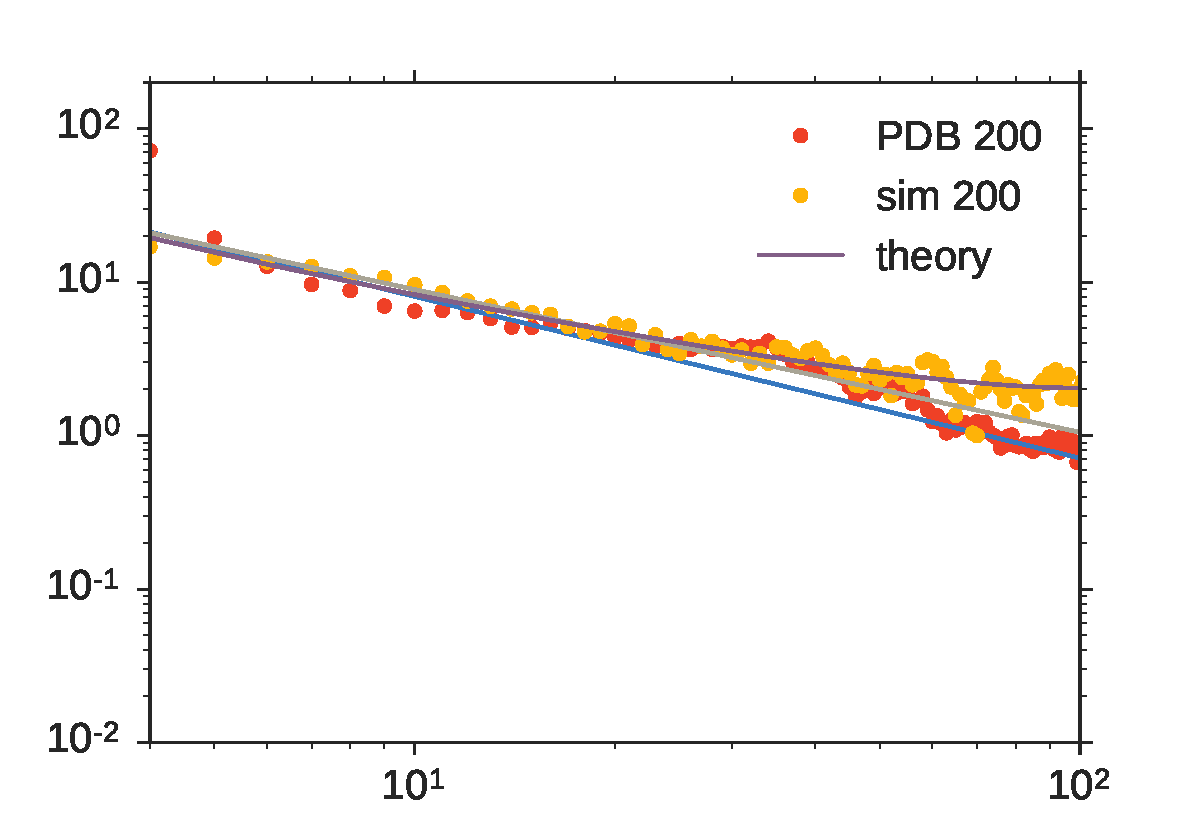
\includegraphics[width=0.45\textwidth]{figures/both_200.pdf}
	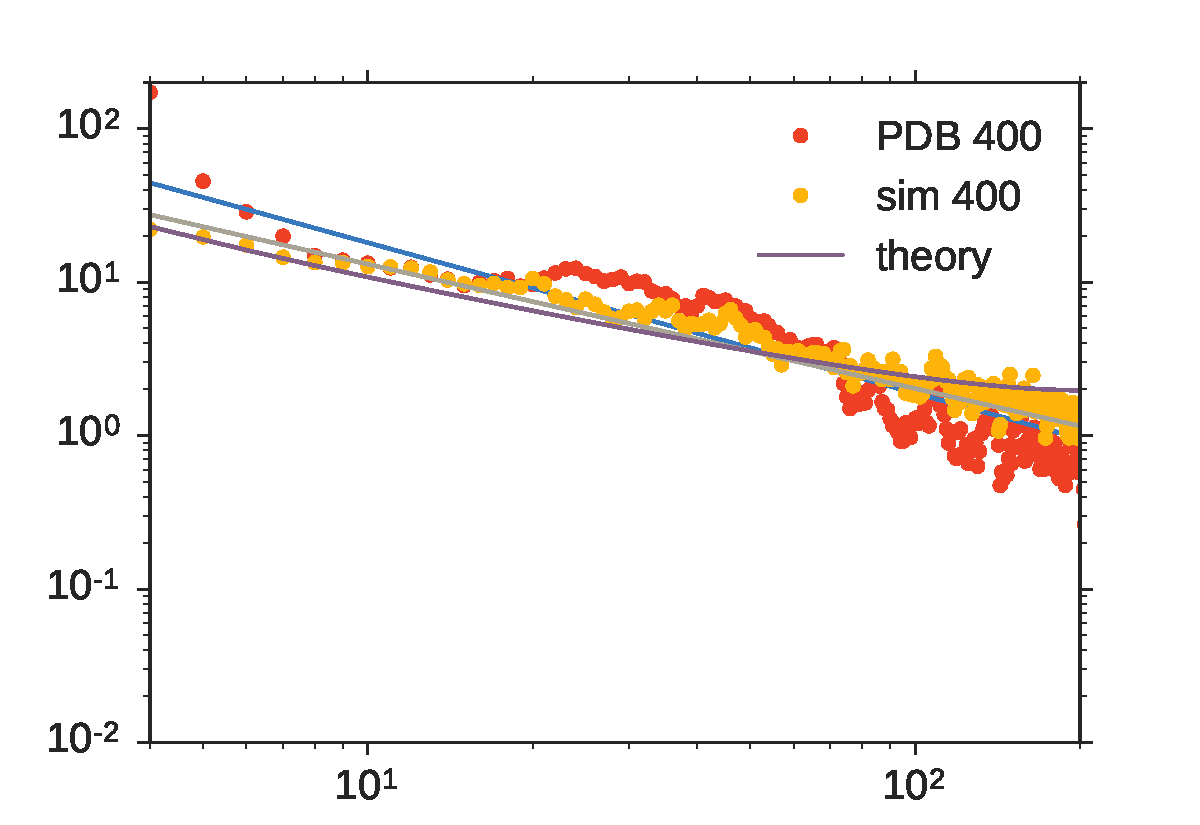
\includegraphics[width=0.45\textwidth]{figures/both_400.pdf}
        \caption{Sequence distance distributions for real and simulated folds for a) Chain lengths around 200 b) chain lengths around 400. The theoretical curve for 2D rings works okay for 3D open chains (because the rings are closed sequence separations of more than N/2 are a bit meaningless and thus not accounted for) The parameters used in this are $A=80$ and $\alpha=0.2$ in a) and $0.3$ in b). I thought in b) it makes sense for $\alpha$ to be larger as there are even larger exponents $k$ coming into relevance. I'm not sure we want to use that whole $\alpha$ argument too much though as it's a but ad-hoc and would be nicer to just fit $A$ and be done with it, but then it may look a bit more off. \red{Redo figure fancier, with more data, axis labels and possibly different lines (remove fit lines, maybe add just one 1/l heuristic line or something).}
        }
        \label{fig:sdd}
\end{figure}
We observe that, while the general shape seems to match, in real proteins sequence separations of 2 to 4 as well as 20 to 50 amino acids are slightly over-represented (see Fig.\ref{fig:sdd}) \red{I have a vague memory of figures with more data where the hump was less pronounced? Depending on this rephrase the above.}.

The over-representation of very short sequence separations is an artefact of the different network construction for simulated networks and PRNs. While in the simulation all links are equally long and links are made until no longer possible, the parameter, determining the connectivity in PRNs is the cutoff distance $d_c$, which is chosen such that the number of links in the PRN is comparable to those in a simulated network of the same $N$. This leads to a larger range of bond angles randomly resulting in connections for small $s$ and thus an over-representation of those links.

\gray{We expect the mid-separation bump to be the result of secondary structure effects. While in the simulation all links are made with equal probability apart from geometric constraints, real protein chains have preferred bond angles leading to the energetic preference for $\alpha-$helix and $\beta-$sheet structures, within which connections only short connections can occur. Longer connections thus tend to be between different helices.
With helices ranging in length from a minimum of about 2 to 3 turns or 7-11 residues up to beyond 30 residues \cite{manning1988circular}, with the (rarer) longer helices accounting relatively for more connections, sequence separations of 20 to 50 seem likely to result from connections between subsequent helices. (I guess we could test this somehow, though i'm not sure how I would go about interpreting the results. I think the PDB files contain information on which residues belong to which structure, so we could do an analysis of how many connections of $s>4$ there are a) within one helix b) between a helix and the following loop) c) between 2 subsequent helices etc. Where I would count helices and sheets the same...)}
\begin{figure}[h]
        \centering
	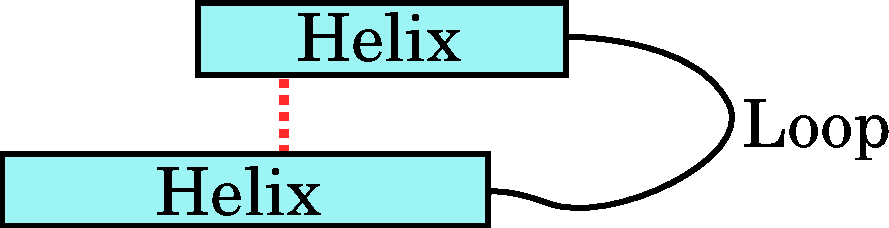
\includegraphics[width=0.35\textwidth]{paper/figures/neighbouring_helices.pdf}
        \caption{\gray{The average length of a link between two subsequent helices is the average length of a helix plus the average length of a loop. \red{Does this suffice or do we want a fancy 3d image of this? If so, do you have the software that makes those?}
        \green{I can make a prettier thing provided we can actually make this argument based on the pdb data. I still struggle make the pdb data comply.}}
        }
        \label{fig:bumpexplain}
\end{figure}

\gray{For a more direct comparison between simulation results and PRNs, we have generated a sample of intrinsically disordered proteins \cite{something}, that also do not contain secondary structures. The results are shown in Fig.~\ref{fig:sdd_idp}.
In order to compare the 3D protein model simulations to PRNs, we selected protein structure lengths based on frequency and comparable length to the simulations. Fig.~\ref{fig:pdb_stats} shows that most proteins in the PDB have chain lengths between 100-400 protein residues. Therefore using example lengths of 200 and 400 residues seemed appropriate. From each of the over 20000 structures around the 200 and 400 residue length, we made the following choices for selecting different types of structures:
...}

\begin{figure}[h]
        \centering
	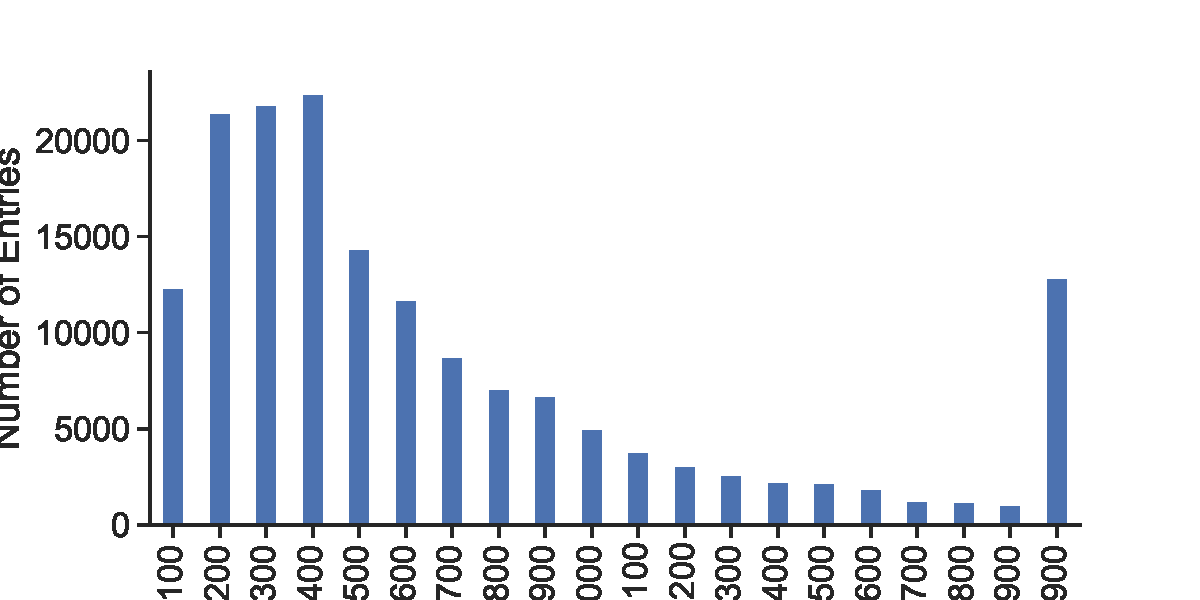
\includegraphics[width=0.45\textwidth]{figures/pdb_statistics.pdf}
        \caption{Statistics on all PDB entries based on the number of amino acid residues, with most entries found in the interval of 100-400 residues as of May 26th 2020. \red{should this figure be before the current fig 2? Because it's the reason we do 200 +- and 400 +-}
        }
        \label{fig:pdb_stats}
\end{figure}

\gray{We find that the over representation of connections with $20<s<50$ disappears, further confirming our expectation.}
\begin{figure}[h]
        \centering
	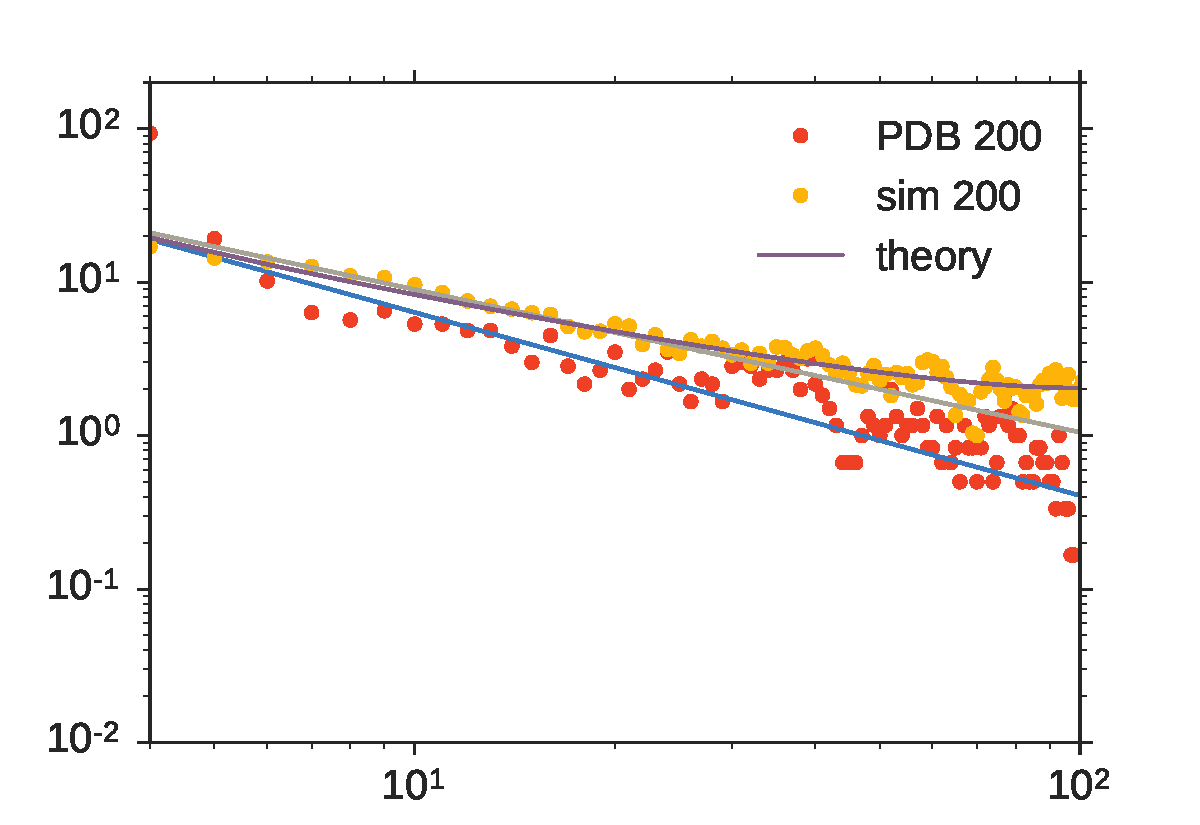
\includegraphics[width=0.45\textwidth]{figures/idp_200.pdf}
	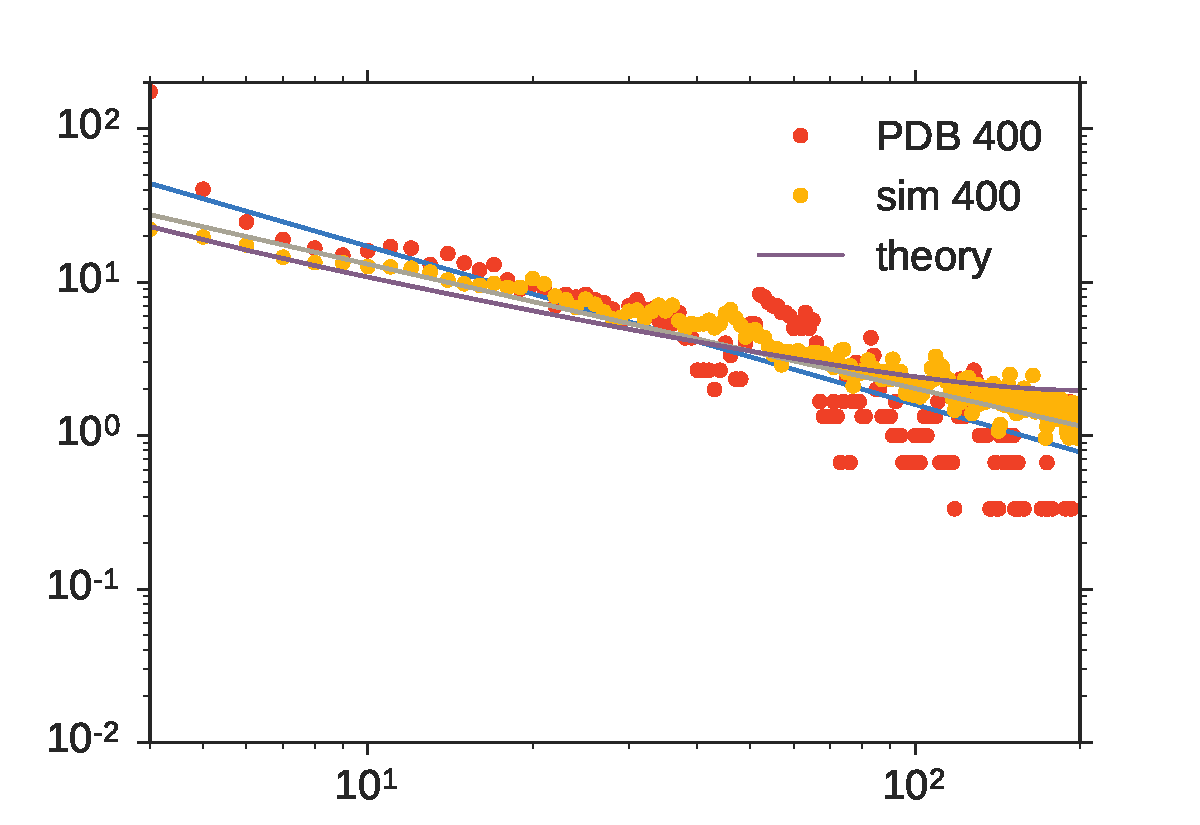
\includegraphics[width=0.45\textwidth]{figures/idp_400.pdf}
        \caption{\gray{Sequence distance distributions for intrinsically disordered proteins and simulated folds for a) Chain lengths around 200 b) chain lengths around 400. The theoretical curve for 2D rings works okay for 3D open chains (because the rings are closed sequence separations of more than N/2 are a bit meaningless and thus not accounted for) The parameters used in this are $A=80$ and $\alpha=0.2$ in a) and $0.3$ in b). I thought in b) it makes sense for $\alpha$ to be larger as there are even larger exponents $k$ coming into relevance. I'm not sure we want to use that whole $\alpha$ argument too much though as it's a but ad-hoc and would be nicer to just fit $A$ and be done with it, but then it may look a bit more off.}
        }
        \label{fig:sdd_idp}
\end{figure}
\red{Anything else we want to say to that? This is a bit short now}
\section*{Conclusion}
We have demonstrated in analytical calculations and direct simulations how a random linking models with geometric constraints, such as the ones introduced in \cite{molkenthin2016scaling, molkenthin2020self} generate sequence distance distributions, that resemble a power-law, similar to the one found in folded proteins. This feature of protein network structure has been used to generate protein-like structures in \cite{bartoli2008effect}.

\red{I remember we agreed on just deleting all the stuff about idp's beause the bump wasn't very pronounced once we used more data and thus the whole narrative of helix lengths and stuff wasn't particularly convincing. Additionally this means less work and thus sooner publication, so we were actually quite happy about it. But then we need to come up with something to write in the conclusion, so far it's a bit short.}

\gray{For proteins with a high percentage of $\alpha$-helix structures, however, we find an over-representation of links with a sequence separation of 20 to 50 residues, implying a higher number of connections between neighbouring helices. We show that this is indeed the case by analyzing the sequence separation distributions of intrinsically disordered proteins. As helix structures arise from local bond angle preferences \cite{Danielsson2010}, rather than geometric constraints, these are not replicated in the model and thus the bump is absent in our theoretical calculations as well as simulations.}

\gray{This makes the sequence separation distribution an indicator for the disorderedness of a protein structure. If such a thing is interesting we could try to formalize this measure and see how good it is at identifying idp's, but i'm guessing they are quite easy to identify already.}

% \begin{enumerate}
%     \item Bartoli et al. made a random network model based on a power-law sequence separation distribution \cite{bartoli2008effect}
%     \item Here we show how such a distribution can be explained directly from geometric constraints
%     \item In the analysis of realistic sequence separation distributions from PRN's we find that the secondary structure leads to an over representation of $20<s<50$, which we can explain as connections between subsequent helices.
%     \item The bump is absent for idp's
%     \item This makes the sequence separation distribution an indicator for the disorderedness of a protein structure. If such a thing is interesting we could try to formalize this measure and see how good it is at identifying idp's, but i'm guessing they are quite easy to identify already.
% \end{enumerate}
\section*{Declarations}
\subsection{Availability of data and materials}
All data generated or analysed during this study are included in this published article [and its supplementary information files].
\subsection{Competing interests}
The authors declare no competing interests.
\subsection{Funding}
This research was supported by ...
\subsection{Authors' contributions}

\subsection{Acknowledgements}
We thank ... for fruitful discussions.

\bibliographystyle{unsrt}
\bibliography{proteins}

\appendix
\section{Supplemental Material Collection}
\section{Random ideas}
\begin{itemize}
    \item Why is the beginning different for simulations?
    \item Does the dip disappear for IDPs
    \item Can we use all NMR structures for IDPs
    \item Would it help using more simulated structures than just the Crystal structure. 
\end{itemize}



\end{document}